\chapter{The Manifold Hypothesis}
\label{chap:manifold}

\section{The Curse and the Blessing of Dimensionality}

The ambient dimension of modern machine learning datasets is staggering. A standard RGB image of size $256 \times 256$ pixels resides in a space of $D = 256 \times 256 \times 3 \approx 200,000$ dimensions. If we were to sample uniformly from this space $\mathcal{X} = [0, 1]^D$, the result would almost always be unstructured static noise. Yet, the images we care about---faces, natural landscapes, handwritten digits---occupy an infinitesimal fraction of this vast ambient space. This striking observation leads us to one of the most fundamental tenets of modern representation learning: the \emph{Manifold Hypothesis}.

The Manifold Hypothesis posits that real-world, high-dimensional data generated by natural processes concentrate on or near a lower-dimensional manifold (or a union of such manifolds) embedded within the high-dimensional ambient space. While the ambient dimension $D$ might be in the millions, the intrinsic dimension $d$ of the data manifold is typically much smaller, constrained by the underlying physical laws and generative factors that gave rise to the data. For instance, the set of all images of a rigid 3D object under various camera angles and lighting conditions forms a low-dimensional topological space, despite each image being a high-dimensional vector.

Understanding the Manifold Hypothesis is crucial for information-theoretic deep learning because it fundamentally resolves a paradox. The classic ``curse of dimensionality'' dictates that the volume of a space grows exponentially with its dimension, meaning that learning a target distribution or function over $\mathbb{R}^D$ should require an exponentially large dataset. If data truly spanned the entirety of $\mathbb{R}^D$, deep neural networks would suffer from catastrophic overfitting, and any attempt to estimate information-theoretic quantities like mutual information $I(X;Y)$ or differential entropy $h(X)$ would be statistically intractable. 

However, deep neural networks routinely circumvent this curse. They do so by exploiting the intrinsic low-dimensional structure of the data. A neural network parameterized by $\theta$ acts as a mapping that warps and folds the ambient space, effectively projecting the data onto representations that linearize the underlying manifold. From an information-theoretic perspective, the network isolates the relevant information bits that define the coordinates on the manifold, while discarding the vast amount of redundant ambient entropy.

\section{Information on a Manifold}

\subsection{Setup and Assumptions}

Let $\mathcal{X} = \mathbb{R}^D$ be the ambient input space. We assume that our dataset $\mathcal{D}$ consists of samples $x_i \sim P_{\text{data}}$, where $P_{\text{data}}$ is a probability measure supported on a compact, smooth Riemannian manifold $\mathcal{M} \subset \mathcal{X}$ of intrinsic dimension $d \ll D$. 

When a continuous random variable $X$ is strictly confined to a lower-dimensional manifold $\mathcal{M}$, it does not admit a probability density function with respect to the standard Lebesgue measure on $\mathbb{R}^D$. Consequently, its standard differential entropy in the ambient space diverges to $-\infty$. To properly measure information, we must define entropy with respect to the volume measure on $\mathcal{M}$.

\begin{definition}[Intrinsic Differential Entropy]
Let $X$ be a random variable distributed according to $P_{\text{data}}$ with support on a $d$-dimensional manifold $\mathcal{M}$. Let $p_{\mathcal{M}}(x)$ denote the density of $X$ with respect to the volume measure $d\mu(x)$ on $\mathcal{M}$. The intrinsic differential entropy is defined as:
\begin{equation}
    h_{\mathcal{M}}(X) = - \int_{\mathcal{M}} p_{\mathcal{M}}(x) \log p_{\mathcal{M}}(x) \, d\mu(x).
\end{equation}
\end{definition}

To relate the continuous manifold to discrete information processing (such as a neural network with finite precision or a dataset with finite samples), we consider the entropy of a quantized version of $X$. 

\subsection{Quantization and Covering Numbers}

\begin{figure}[ht]
    \centering
    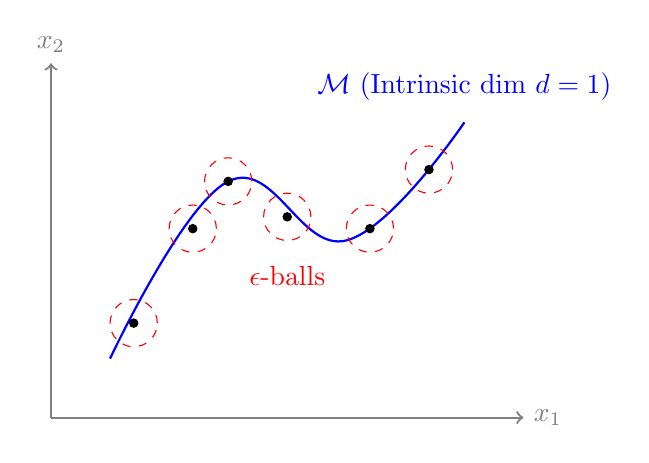
\begin{tikzpicture}[scale=1.5]
        % Ambient space axes
        \draw[->, thick, gray] (0,0) -- (4,0) node[right] {$x_1$};
        \draw[->, thick, gray] (0,0) -- (0,3) node[above] {$x_2$};
        
        % Manifold curve
        \draw[thick, blue, smooth, tension=0.7] plot coordinates {(0.5, 0.5) (1.5, 2.0) (2.5, 1.5) (3.5, 2.5)};
        \node[blue] at (3.5, 2.8) {$\mathcal{M}$ (Intrinsic dim $d=1$)};
        
        % Data points and epsilon tubes
        \foreach \x/\y in {0.7/0.8, 1.2/1.6, 1.5/2.0, 2.0/1.7, 2.7/1.6, 3.2/2.1} {
            \filldraw[black] (\x,\y) circle (1pt);
            \draw[red, dashed] (\x,\y) circle (0.2);
        }
        
        \node[red] at (2.0, 1.2) {$\epsilon$-balls};
    \end{tikzpicture}
    \caption{A $d=1$ dimensional manifold embedded in a $D=2$ dimensional ambient space. The data is quantized by covering the manifold with $\epsilon$-balls, revealing its intrinsic dimension rather than the ambient dimension.}
    \label{fig:manifold_cover}
\end{figure}

Consider covering the space with hypercubes (or balls) of diameter $\epsilon$. Let $X^\epsilon$ denote the discrete random variable obtained by quantizing $X$ to the centers of these $\epsilon$-bins. As $\epsilon \to 0$, the standard relationship in $\mathbb{R}^D$ is $H(X^\epsilon) \approx h(X) - D \log \epsilon$. However, when $X$ is constrained to $\mathcal{M}$, the growth rate of the discrete entropy depends solely on the intrinsic dimension $d$.

\begin{theorem}[Quantization Entropy on a Manifold]
Let $X \sim P_{\text{data}}$ have support on a $d$-dimensional compact manifold $\mathcal{M} \subset \mathbb{R}^D$ and possess a well-defined intrinsic differential entropy $h_{\mathcal{M}}(X)$. Let $X^\epsilon$ be the $\epsilon$-quantization of $X$. As $\epsilon \to 0$, the discrete Shannon entropy of $X^\epsilon$ satisfies:
\begin{equation}
    H(X^\epsilon) = h_{\mathcal{M}}(X) - d \log \epsilon + \mathcal{O}(1).
\end{equation}
\end{theorem}

\begin{proof}
Let $N(\epsilon)$ be the $\epsilon$-covering number of the manifold $\mathcal{M}$, defined as the minimum number of balls of radius $\epsilon$ required to completely cover $\mathcal{M}$. Since $\mathcal{M}$ is a compact $d$-dimensional manifold, its volume scales with dimension $d$. Specifically, the covering number behaves as:
\begin{equation}
    N(\epsilon) \approx \frac{\text{Vol}(\mathcal{M})}{C_d \epsilon^d}
\end{equation}
where $C_d$ is the volume of a $d$-dimensional unit ball. 

Let the quantized bins intersecting $\mathcal{M}$ be indexed by $i = 1, \dots, N(\epsilon)$. The probability of the $i$-th bin is $p_i = \int_{\text{bin}_i} p_{\mathcal{M}}(x) \, d\mu(x)$. By the mean value theorem for integration, $p_i \approx p_{\mathcal{M}}(x_i) \Delta V_i$, where $x_i$ is a point in the $i$-th bin and $\Delta V_i \approx C_d \epsilon^d$ is the intersection volume of the bin with the manifold.

The discrete entropy is:
\begin{align*}
    H(X^\epsilon) &= - \sum_{i=1}^{N(\epsilon)} p_i \log p_i \\
    &\approx - \sum_{i=1}^{N(\epsilon)} p_{\mathcal{M}}(x_i) \Delta V_i \log \left( p_{\mathcal{M}}(x_i) C_d \epsilon^d \right) \\
    &= - \sum_{i=1}^{N(\epsilon)} p_{\mathcal{M}}(x_i) \log(p_{\mathcal{M}}(x_i)) \Delta V_i - \log(C_d \epsilon^d) \sum_{i=1}^{N(\epsilon)} p_{\mathcal{M}}(x_i) \Delta V_i \\
    &\approx h_{\mathcal{M}}(X) - \log(C_d \epsilon^d) \cdot 1 \\
    &= h_{\mathcal{M}}(X) - d \log \epsilon - \log C_d.
\end{align*}
As $\epsilon \to 0$, the approximation becomes exact, and the $\mathcal{O}(1)$ term corresponds to $-\log C_d$ and boundary effects. This concludes the proof.
\end{proof}

This theorem provides a rigorous foundation for why representation learning is possible. The number of bits required to encode the data to a precision $\epsilon$ scales linearly with $d$, not $D$. Deep learning models act as adaptive quantizers that effectively discover this $d$-dimensional coordinate system.

\subsection{Numerical Example: Estimating Intrinsic Dimension}

Suppose data is distributed uniformly on the surface of a 2-sphere $S^2$ of radius $R=1$, embedded in $\mathbb{R}^3$. The ambient dimension is $D=3$. The intrinsic dimension is $d=2$. The volume (surface area) is $\text{Vol}(S^2) = 4\pi$.

Because the distribution is uniform, the intrinsic density is $p_{\mathcal{M}}(x) = \frac{1}{4\pi}$. The intrinsic differential entropy is:
\begin{equation}
    h_{\mathcal{M}}(X) = - \int_{S^2} \frac{1}{4\pi} \log \left(\frac{1}{4\pi}\right) d\mu(x) = \log(4\pi).
\end{equation}
If we quantize the space with a grid of resolution $\epsilon$, the number of bins covering the sphere will grow proportionally to $1/\epsilon^2$. The discrete entropy of the quantized data $X^\epsilon$ will be $H(X^\epsilon) \approx \log(4\pi) - 2 \log \epsilon$. If we mistakenly attempted to measure the entropy in $\mathbb{R}^3$, the differential entropy $h(X)$ would evaluate to $-\infty$, because the 3D volume of the sphere's surface is zero.

\subsection{Representational Unfolding}

A neural network $f_\theta: \mathcal{X} \to \mathcal{Z}$ can be understood geometrically as a sequence of homeomorphisms that "unfold" the manifold $\mathcal{M}$ into a flat Euclidean space, facilitating linear separability for downstream classification tasks.

\begin{figure}[ht]
    \centering
    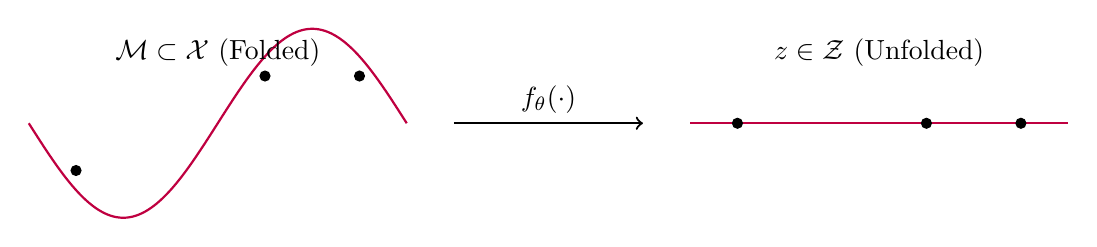
\begin{tikzpicture}[scale=1.2]
        % Input manifold (folded)
        \draw[thick, purple] (0,2) sin (1,1) cos (2,2) sin (3,3) cos (4,2);
        \node[above] at (2,2.5) {$\mathcal{M} \subset \mathcal{X}$ (Folded)};
        
        % Arrow mapping
        \draw[->, thick] (4.5, 2) -- (6.5, 2) node[midway, above] {$f_\theta(\cdot)$};
        
        % Output representation (unfolded)
        \draw[thick, purple] (7,2) -- (11,2);
        \node[above] at (9,2.5) {$z \in \mathcal{Z}$ (Unfolded)};
        
        % Data points
        \filldraw[black] (0.5, 1.5) circle (1.5pt);
        \filldraw[black] (2.5, 2.5) circle (1.5pt);
        \filldraw[black] (3.5, 2.5) circle (1.5pt);
        
        \filldraw[black] (7.5, 2) circle (1.5pt);
        \filldraw[black] (9.5, 2) circle (1.5pt);
        \filldraw[black] (10.5, 2) circle (1.5pt);
    \end{tikzpicture}
    \caption{A deep neural network $f_\theta$ maps the complex, highly folded data manifold in the ambient space $\mathcal{X}$ into a flattened, linearly interpolable latent space $\mathcal{Z}$.}
    \label{fig:manifold_unfolding}
\end{figure}

The success of architectures like ResNets can be attributed to their ability to learn diffeomorphisms of the ambient space that iteratively flatten $\mathcal{M}$. The Information Bottleneck principle (discussed in later chapters) formally dictates how much of the ambient space's irrelevant entropy is discarded during this unfolding process.

\begin{horizon}
It is conjectured that the dynamics of Stochastic Gradient Descent (SGD) inherently bias neural networks toward discovering and aligning with the lowest-dimensional manifold that sufficiently explains the training data. While we have proven that the minimum encoding length scales with the intrinsic dimension $d$, an open question is whether the implicit regularization of modern deep learning optimizers perfectly mirrors a search for minimal intrinsic capacity.

Future work might show that the layer-wise transformations in sufficiently overparameterized networks perfectly correspond to the principal curvatures of the data manifold. Furthermore, it remains conjectured that the generalization gap in deep learning can be entirely bounded by the topological complexity (e.g., the Betti numbers) of the data manifold relative to the network's capacity. Proving these claims would require bridging differential geometry with the non-equilibrium thermodynamics of gradient descent, a synthesis that currently remains out of reach.
\end{horizon}

\section{Summary}
In this chapter, we formalized the Manifold Hypothesis, demonstrating why high-dimensional datasets are mathematically tractable. By differentiating between ambient dimension $D$ and intrinsic dimension $d$, we showed that the discrete entropy of quantized data scales with $d$, effectively bypassing the curse of dimensionality. We rigorously defined intrinsic differential entropy and proved its relationship with quantization. The geometry of the data manifold dictates the minimum information rate required to represent the data, setting the stage for analyzing neural networks as mechanisms that compress and unfold these topological structures.

\section*{Exercises}
\begin{enumerate}
    \item \textbf{Intrinsic vs. Ambient Divergence:} Suppose two distributions $P$ and $Q$ have support on the same 1D manifold (a circle) embedded in $\mathbb{R}^2$. Prove that their Kullback-Leibler divergence $D_{\text{KL}}(P \parallel Q)$ computed using their intrinsic 1D densities is equivalent to the limit of the KL divergence between their $\epsilon$-noisy ambient representations as $\epsilon \to 0$.
    \item \textbf{Entropy of a Line Segment:} Let $X$ be distributed uniformly on a line segment of length $L$ embedded in $\mathbb{R}^3$. Calculate the intrinsic differential entropy $h_{\mathcal{M}}(X)$. Then, derive the exact discrete entropy $H(X^\epsilon)$ for a 1D uniform grid quantization and compare it with the asymptotic formula $H(X^\epsilon) \approx h_{\mathcal{M}}(X) - \log \epsilon$.
    \item \textbf{Manifold Noise:} Consider data strictly on a manifold, $X \sim P_{\text{data}}$, and noisy observations $Y = X + \epsilon Z$, where $Z \sim \mathcal{N}(0, I_{D})$. As $D \to \infty$, explain the information-theoretic difficulty of estimating the intrinsic dimension $d$ from finite samples of $Y$, invoking the concept of ambient noise.
\end{enumerate}

% TODO-CITE: Ensure all named results are cited.
